

\begin{figure*}[!t] \center
	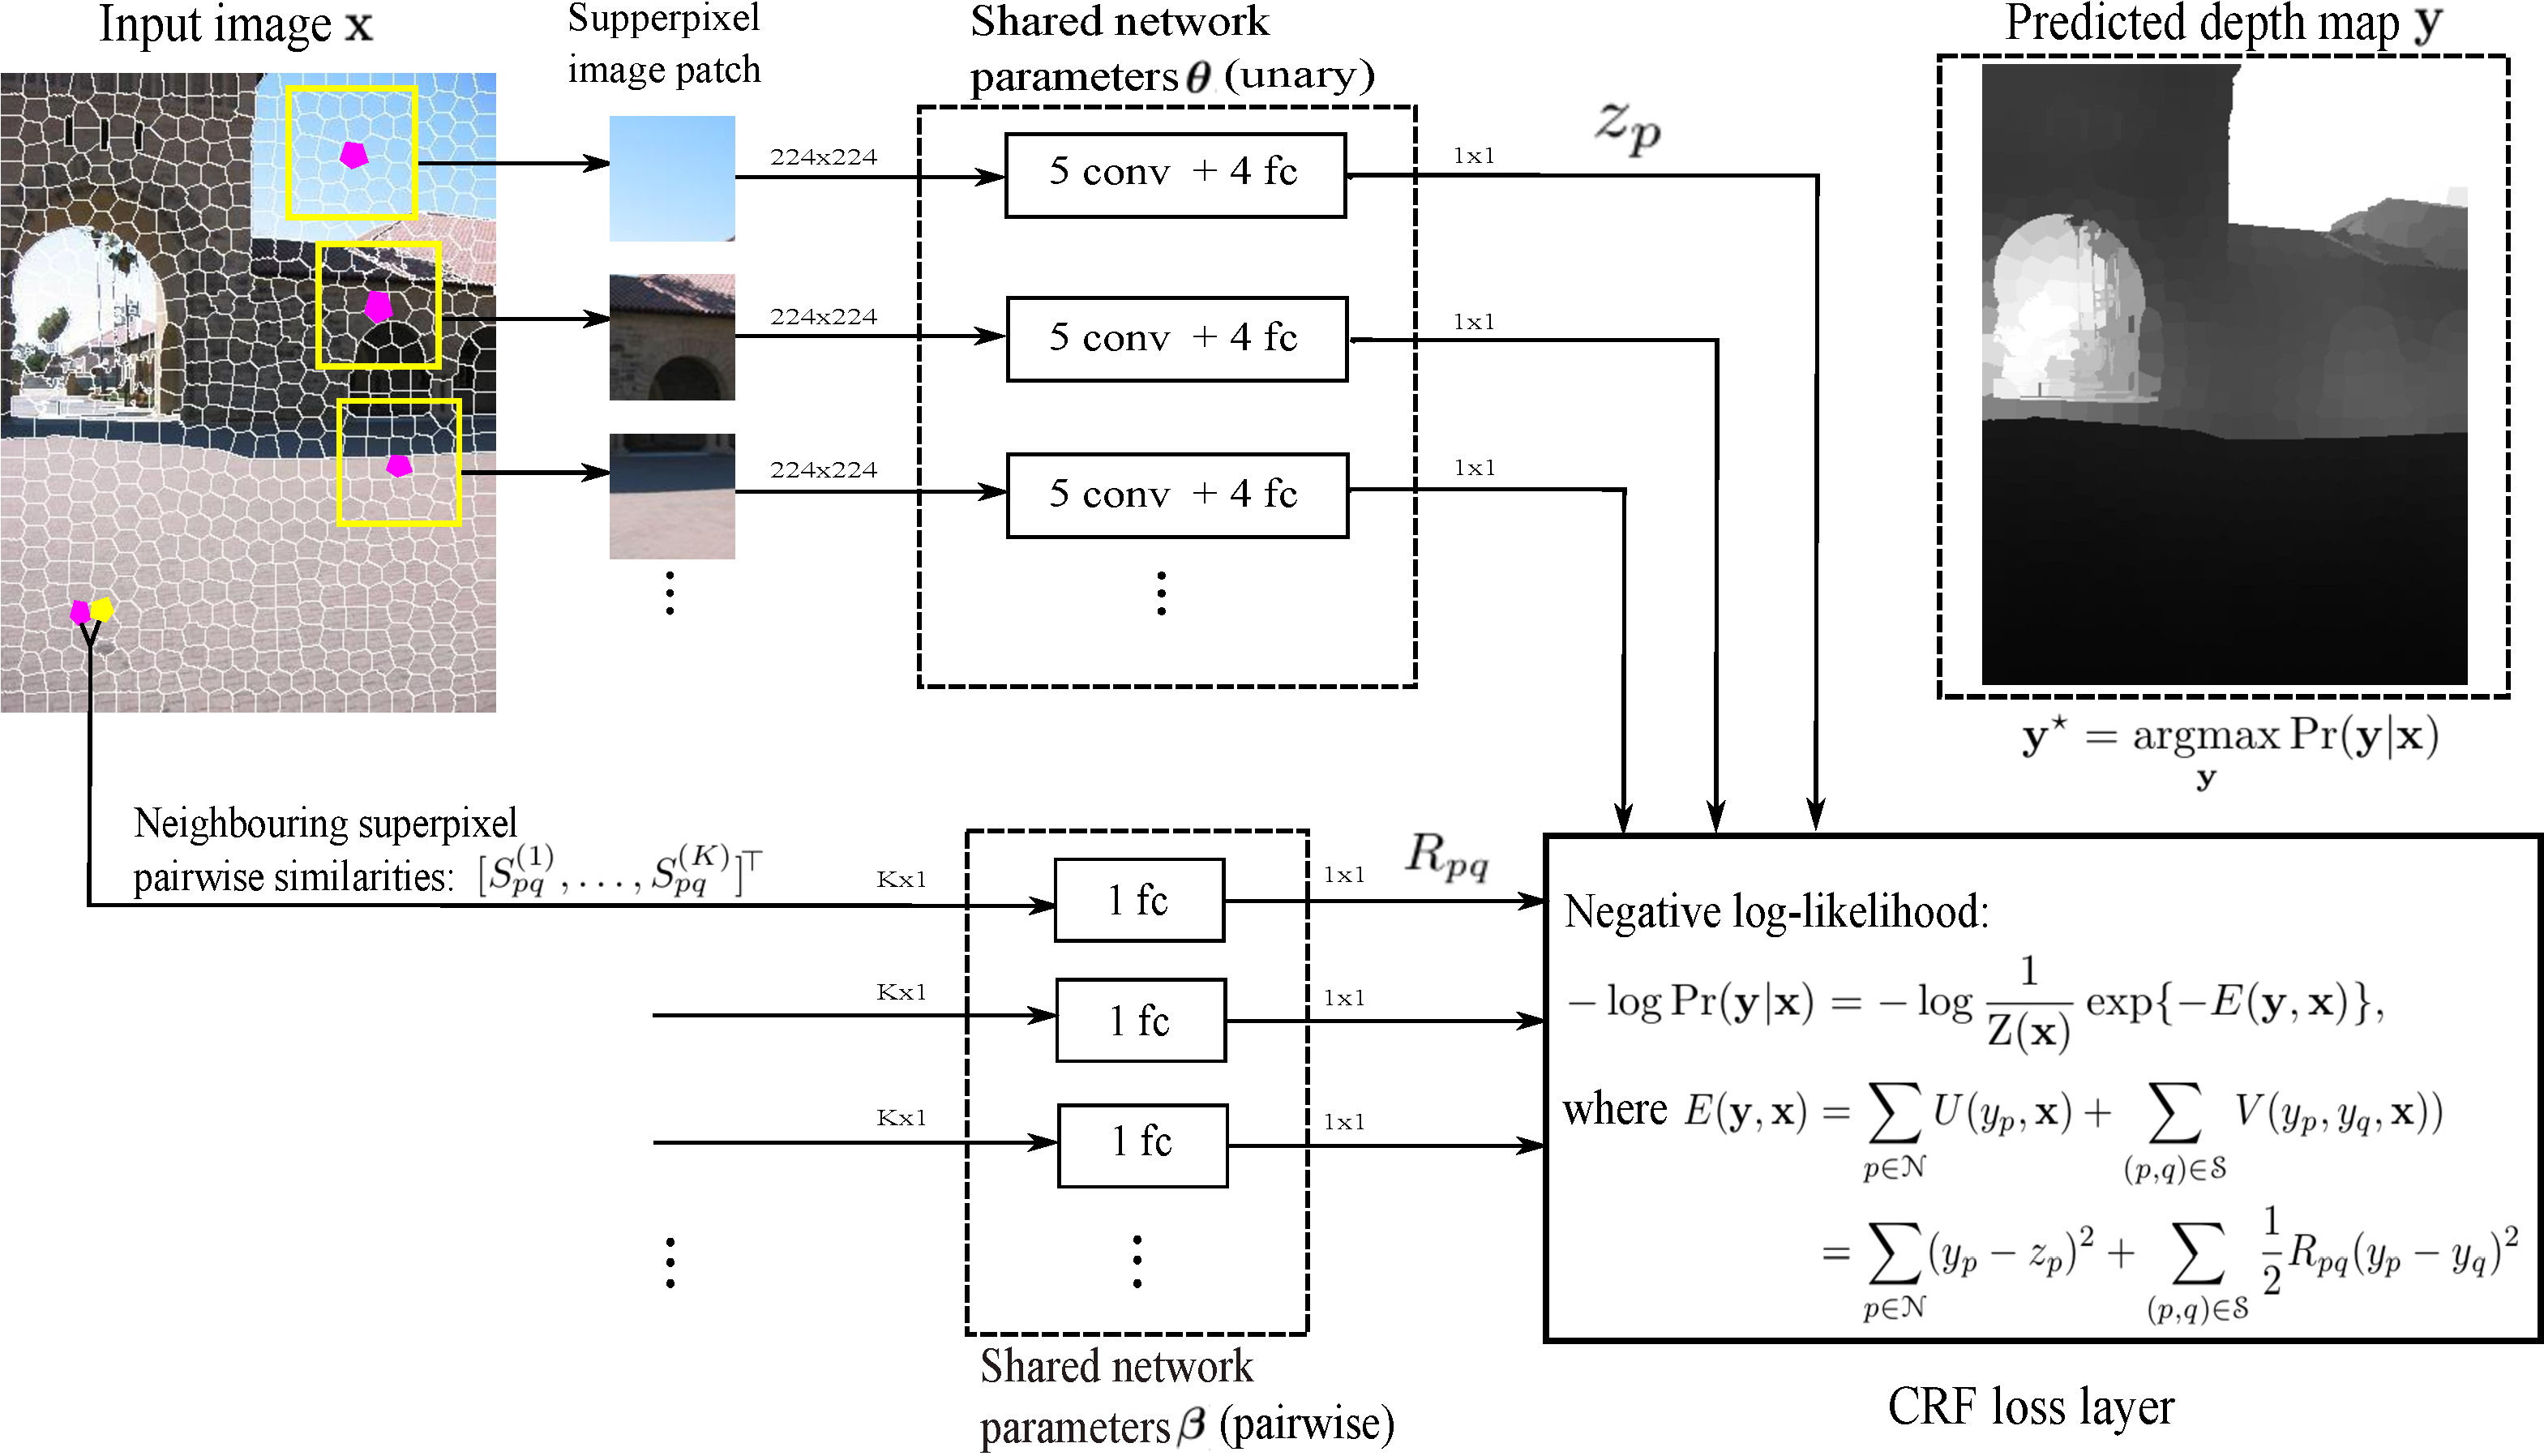
\includegraphics[width=0.88\textwidth]{./fig/cnn_network.pdf}
\caption{An illustration of our deep convolutional neural field model for depth estimation. 
The input image is first over-segmented into superpixels. 
In the unary part, for a superpixel $p$, we crop the image patch centred around its centroid, 
%
then resize and feed it to a \cnn which is composed of 5 convolutional and 4 fully-connected layers (details refer to Fig. \ref{fig:cnn_unary}).
In the pairwise part,
for a pair of neighbouring superpixels $(p, q)$, we consider $K$ types of similarities, and feed them into a fully-connected layer. 
The outputs of unary part and the pairwise part are then fed to the \crf structured loss layer, which minimizes the negative log-likelihood.     
Predicting the depths of a new image $\x$ is to maximize the conditional probability $\Pr(\y|\x)$, which has closed-form solutions (see Sec. \ref{sec:learning} for details).
}  \label{fig:cnn_ccrf}
\end{figure*}






%
\section{Deep convolutional neural fields}



%
We present the details of our deep convolutional neural field model for depth estimation in this section. Unless otherwise stated, we use boldfaced uppercase and lowercase letters to denote matrices and column vectors respectively.
%


%
\subsection{Overview}
The goal here is to infer the depth of each pixel in a single image depicting general scenes. 
Following the work of \cite{make3d_pami09,Liu_cvpr12,Miaomiao_cvpr14}, 
we make the common assumption that an image is composed of small homogeneous regions (superpixels)   
and consider the graphical model composed of nodes defined on superpixels.
Kindly note that our framework is flexible that can work on pixels or superpixels.
Each superpixel is portrayed by the depth of its centroid.
Let $\x$ be an image and $\y=[y_1,\ldots, y_n]^{\T} \in \Real^n$ be 
%
a vector of continuous depth values corresponding to
 all $n$ superpixels in $\x$. 
 %
 Similar to conventional CRF,
 we model the conditional probability distribution of the data with the following density function:
%
\begin{equation}\label{eq:prob}
\begin{aligned}
\Pr(\y|\x) = \frac{1}{\mathrm{Z(\x)}} \exp (- E(\y, \x)),
\end{aligned}
\end{equation}
where $E$ is the energy function; $\mathrm{Z}$ is the partition function  defined as:
\begin{equation}\label{eq:partition}
\mathrm{Z}(\x) = \int_{\y} \exp \{ -E(\y, \x) \}\mathrm{d}\y.
\end{equation}
Here, because $\y$ is continuous, the integral in Eq. \eqref{eq:prob} can be analytically calculated under certain circumstances, which we will show in Sec. \ref{sec:learning}.
This is different from the discrete case, in which approximation methods need to be applied.  
To predict the depths of a new image, we solve the maximum a posteriori (MAP) inference problem: 
\begin{align} \label{eq:inference}
\y^{\star}&=\argmax_{\y} \Pr(\y|\x). 
\end{align} 




\begin{figure*}[!t] \center
	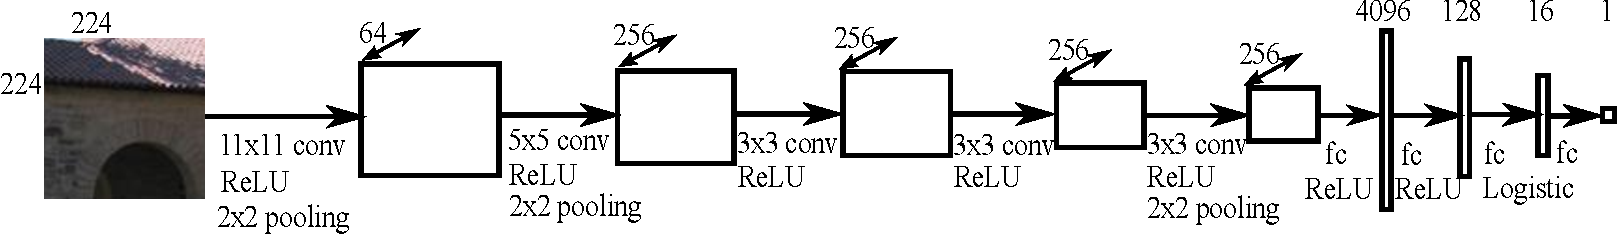
\includegraphics[width=0.85\textwidth]{./fig/cnn_unary.pdf}
\caption{Detailed network architecture of the unary part in Fig. \ref{fig:cnn_ccrf}. }  \label{fig:cnn_unary}
\end{figure*}




We formulate the energy function as a typical combination of unary potentials $U$ and pairwise potentials $V$ over the nodes (superpixels) $\cal N$ and edges $\cal S$ of the image $\x$:
\begin{equation}\label{eq:energy}
E(\y, \x) = \sum_{p \in {\cal N} } U(y_{p}, \x) 
	 + \sum_{(p,q) \in {\cal S}} V(y_{p}, y_{q}, \x).
\end{equation}
The unary term $U$ aims to regress the depth value from a single superpixel. 
The pairwise term $V$ encourages neighbouring superpixels with similar appearances to take similar depths.
We aim to jointly learn $U$ and $V$ in a unified \cnn framework.

In Fig. \ref{fig:cnn_ccrf}, we show a sketch of our 
%
deep convolutional neural field model
for depth estimation.   
As we can see, the whole network is composed of a unary part, a pairwise part and a \crf loss layer.
For an input image, which has been over-segmented into $n$ superpixels, 
we consider image patches centred around each superpxiel centroid.
%
The unary part then takes  all the image patches as input and feed each of them to a \cnn 
and output an $n$-dimentional vector containing regressed depth values of the $n$ superpixels. 
The network for the unary part is composed of $5$ convolutional and $4$ fully-connected layers with details in Fig. \ref{fig:cnn_unary}. Kindly note that the \cnn parameters are shared across all the superpixels. 
The pairwise part %
takes similarity vectors (each with $K$ components)  of all neighbouring superpixel pairs as input and feed each of them to a fully-connected layer (parameters are shared among different pairs), then output a vector containing all the $1$-dimentional similarities for each of the neighbouring superpixel pair.
The \crf loss layer takes as input the outputs from the unary and the pairwise parts to minimize the negative log-likelihood.
Compared to the direct regression method in \cite{dcnn_nips14}, 
%
our model possesses two potential advantages: 
1) We achieve translation invariance as we construct unary potentials irrespective of the superpixel's coordinate (shown in Sec. \ref{sec:potentials});  
2) We explicitly model the relations of neighbouring superpixels through pairwise potentials.

 

In the following, we describe the details of potential functions involved in the energy function in Eq. \eqref{eq:energy}.








\subsection{Potential functions}
\label{sec:potentials}

\paragraph{Unary potential}
The unary potential is constructed from the output of a \cnn by considering the least square loss:
\begin{equation}\label{eq:unary}
U(y_{p}, \x;\btheta) = (y_p - \regress_p (\btheta))^2, \;\; \forall p=1,...,n.
\end{equation}
Here $\regress_p$ is the regressed depth of the superpixel $p$ parametrized by the \cnn parameters $\btheta$.
%

The network architecture for the unary part is depicted in Fig. \ref{fig:cnn_unary}.
Our \cnn model in Fig. \ref{fig:cnn_unary} is mainly based upon the well-known network architecture of Krizhevsky \etal \cite{AlexNet12} with modifications. 
It is composed of $5$ convolutional layers and $4$ fully connected layers. 
The input image is first over-segmented into superpixels, then for each superpixel, we consider the image patch centred around its centroid. Each of the image patches is resized to $ 224 \times 224$ pixels and then fed to the convolutional neural network.
Note that the convolutional and the fully-connected layers are shared across all the image patches of different superpixels. 
Rectified linear units (ReLU) are used as activiation functions for the five convolutional layers and the first two fully connected layers. 
For the third fully-connected layer, we use the logistic function ($f(x)=(1+e^{-x})^{-1}$) as activiation function.
%
The last fully-connected layer plays the role of model ensemble with no activiation function followed. 
The output is an $1$-dimentional real-valued depth for a single superpixel.  










\paragraph{Pairwise potential}
We construct the pairwise potential from $K$ types of similarity observations, each of which enforces smoothness by exploiting consistency information of neighbouring superpixels:
\begin{align} \label{eq:pairwise}
&V(y_{p}, y_{q}, \x; \bbeta) = \half \pws_{pq} (y_p - y_q)^2, \;\forall p,q=1,...,n.
%
\end{align}
Here $\pws_{pq}$ is the output of the network in the pairwise part (see  Fig. \ref{fig:cnn_ccrf}) from a neighbouring superpixel pair $(p,q)$. 
We use a fully-connected layer here:
\begin{align}  \label{eq:def_R}
\pws_{pq} = \bbeta^{\T} [S_{pq}^{(1)},\ldots,S_{pq}^{(K)}]^{\T} = \sum_{k=1}^K \beta_k S_{pq}^{(k)},
\end{align} 
where $\S^{(k)}$ is the $k$-th similarity matrix whose elements are $S_{pq}^{(k)}$ ($\S^{(k)}$ is symmetric);
$\bbeta=[\beta_1, \ldots, \beta_k]^{\T}$ 
are the network parameters.
From Eq. \eqref{eq:def_R}, we can see that we don't use any activiation function.
However, as our framework is general, more complicated networks can be seamlessly incorporated for the pairwise part.
In Sec .\ref{sec:learning}, we will show that we can derive a general form for calculating the gradients with respect to $\bbeta$ (see Eq. \eqref{eq:derive_beta_final}).  
%
%
%
%
To guarantee 
%
$Z(x)$ (Eq. \eqref{eq:partition}) is integrable, we require $\beta_k \geq 0$ \cite{ccrf_nips08}.
%


We consider $3$ types of pairwise similarities, measured by the color difference, color histogram difference and texture disparity in terms of local binary patterns (LBP) \cite{LBP_icpr94}, which take the conventional form: 
%
$S_{pq}^{(k)} = e^{-\gamma \norm{s_p^{(k)} - s_q^{(k)}}}, k=1,2,3$,
where $s_p^{(k)}$, $s_q^{(k)}$ are the observation values of the superpixel $p$, $q$ calculated from color, color histogram and LBP; 
$\norm{\cdot}$ denotes the $\ell_2$ norm of a vector and $\gamma$ is a constant.



%
%
%

 
%
%
%
%
%
%
%
%
%
%
%
%
%
%
%
%









\subsection{Learning}
\label{sec:learning}
With the unary and the pairwise pontentials defined in Eq. \eqref{eq:unary}, \eqref{eq:pairwise}, we can now write the energy function as:
\begin{equation}\label{eq:feature}
E(\y, \x) = \sum_{p \in {\cal N} } (y_p - \regress_p)^2 
+ \sum_{(p,q) \in {\cal S}} \half \pws_{pq} (y_p - y_q)^2.
\end{equation}
For ease of expression, we introduce the following notation: 
\begin{align} \label{eq:def_Amat}
 \A = \I+ \D - \bpws, 
\end{align}
%
%
%
where $\I$ is the $ n \times n$ identity matrix; $\bpws$ is the matrix composed of $\pws_{pq}$;  $\D$ is a diagonal matrix with $\D_{pp} = \sum_q \pws_{pq}$.
Expanding Eq. \eqref{eq:feature}, we have:
\begin{align} \label{eq:feature_expand}
E(\y, \x) = \y^\T \A \y - 2\bregress^\T \y + \bregress^\T \bregress.
\end{align}
Due to the quadratic terms of $\y$ in the energy function in Eq. \eqref{eq:feature_expand} and the positive definiteness of $\A$, we can analytically calculate the integral in the partition function (Eq. \eqref{eq:partition}) as:
\begin{align} \label{eq:partition_expand}
Z(\x) &= \int_{\y} \exp \{ -E(\y, \x) \}\mathrm{d}\y  \notag \\
 	&=\frac{{(\pi)}^{\frac{n}{2}}}{{|\A|}^{\frac{1}{2}}} \exp \{{ \bregress ^\T \A^{-1} \bregress} - \bregress^\T \bregress \}.
\end{align}
From Eq. \eqref{eq:prob}, \eqref{eq:feature_expand},  \eqref{eq:partition_expand},  we can now write the probability distribution function as (see supplementary for details):
\begin{align} \label{eq:prob_final}
\Pr(\y|\x) =\frac{ |\A|^{\half}} {{\pi^{\frac{n}{2}}}} \exp \Big\{ - \y^\T \A \y + 2\bregress^\T \y -  \bregress ^\T \A^{-1} \bregress \Big\}, 
\end{align}
where $\bregress=[\regress_1, \ldots, \regress_n]^{\T}$; $|\A|$ denotes the determinant of the matrix $\A$, and $\A^{-1}$ the inverse of $\A$.
Then the negative log-likelihood can be written as:
\begin{align} \label{eq:log-likelihood}
-\log\Pr(\y|\x)&= \y^\T \A \y - 2\bregress^\T \y + \bregress ^\T \A^{-1} \bregress  \\ \notag
& - \half\log(|\A|) + \frac{n}{2}\log(\pi). 
\end{align}



%
%
%
%
%
%
%
%
%
%
%
%
%
During learning, we minimizes the negative conditional log-likelihood of the training data. Adding regularization to $\btheta$, $\bbeta$, we then arrive at the final optimization:
\begin{align} \label{eq:ccrf_final}
\min_{\btheta, \bbeta \geq \zeros} &-\sum_{i=1}^N \log\Pr(\y^{(i)} | \x^{(i)}; \btheta, \bbeta) \\ \notag 
&+ \frac{\lambda_1}{2} \fnorm \btheta + \frac{\lambda_2}{2} \fnorm \bbeta,
\end{align} 
where $\x^{(i)}$, $\y^{(i)}$ denote the $i$-th training image and the corresponding depth map; $N$ is the number of training images; $\lambda_1$ and $\lambda_2$ are weight decay parameters.
We use stochastic gradient descent (SGD) based back propagation to solve the optimization problem in Eq.  \eqref{eq:ccrf_final} for learning all parameters of the whole network.
%
We project the solutions to the feasible set when the bounded constraints $\beta_k \geq 0$ is violated.
In the following, we calculate the partial derivatives of $-\log\Pr(\y|\x)$ with respect to the network parameters $\theta_l$ (one element of $\btheta$) and $\beta_k$ (one element of $\bbeta$) by using the chain rule (refer to supplementary for details): 
%
\begin{align}   
\frac{\partial \{ -\log\Pr(\y|\x)\} }{\partial \theta_l} 
%
%
%
& = 2 (\A^{-1} \bregress - \y)^{\T} \frac{\partial \bregress}{\partial \theta_l}, \label{eq:derive_z} \\
%
%
\frac{\partial \{ -\log\Pr(\y|\x)\} }{\partial \beta_k} 
& = \y^{\T} \J \y - \bregress^{\T} \A^{-1} \J \A^{-1}\bregress \notag \\
& \; - \half \trace \Big( \A^{-1} \J \Big),  \label{eq:derive_beta_final}
\end{align}
%
%
%
%
%
%
%
where $\trace(\cdot)$ denotes the trace of a matrix; $\J$ is an $n \times n$ matrix with elements:
\begin{align}  \label{eq:def_J}
J_{pq}& =  - \frac{\partial  \pws_{pq} }{\partial \beta_k} 
+ \delta(p=q) \sum_q \frac{\partial  \pws_{pq} }{\partial \beta_k}, 
\end{align}
where $\delta(\cdot)$ is the indicator function, which equals 1 if $p=q$ is true and 0 otherwise. 
From Eq. \eqref{eq:def_J}, we can see that our framework is general and more complicated networks for the pairwise part can be seamlessly incorporated.
Here, in our case, with the definition of $\pws_{pq}$ in Eq. \eqref{eq:def_R}, we have $\frac{\partial  \pws_{pq} }{\partial \beta_k}=S_{pq}^{(k)}$.
%
%
%
%
%
%
%
%
%
%
%
%



\paragraph{Depth prediction}
Predicting the depths of a new image is to solve the MAP inference in Eq. \eqref{eq:inference}, in which closed form solutions exist here (details refer to supplementary): %
\begin{align} \label{eq:inf_solution}
\y^{\star}&=\argmax_{\y} \Pr(\y|\x)  \\ \notag
&= \argmax_{\y} -\y^\T \A \y + 2\bregress^\T \y  \\  \notag
&= \A^{-1} \bregress.
\end{align} 
If we discard the pairwise terms, namely $\pws_{pq}=0$, then Eq. \eqref{eq:inf_solution} degenerates to $\y^{\star}=\bregress$, which is a conventional regression model (we will report the results of this method as a baseline in the experiment). 


%
%


%












\subsection{Implementation details}
We implement the network training based on the efficient CNN toolbox: VLFeat MatConvNet\footnote{VLFeat MatConvNet: http://www.vlfeat.org/matconvnet/} \cite{matconvnet}. 
Training is done on a standard desktop with an NVIDIA GTX 780 GPU with 6GB memory. 
%
%
During each SGD iteration, around $\sim 700$ superpixel image patches need to be processed.
The 6GB GPU may not be able to process all the image patches at one time.
We therefore partition the superpixel image patches of one image into two parts and process them successively.
%
%
%
%
Processing one image takes around $10$s (including forward and backward) with $\sim 700$ superpixels when training the whole network.


During implementation, we initialize the first 6 layers of the unary part in Fig. \ref{fig:cnn_unary} using a \cnn model trained on the ImageNet from \cite{vgg_bmvc14}.
First, we do not back propagate through the previous 6 layers by keeping them fixed and train the rest of the network (we refer this process as pre-train) with the following settings: 
%
momentum is set to $0.9$, and weight decay parameters $\lambda_1, \lambda_2$ are set to $0.0005$.
During pre-train, the learning rate is initialized at $0.0001$,
and decreased by 40\% every 20 epoches. 
%
%
We then run 60 epoches to report the results of pre-train (with learning rate decreased twice).
The pre-train is rather efficient, taking around $1$ hour to train on the Make3D dataset, and inferring the depths of a new image takes less than $0.1$s.
Then we train 
%
the whole network with the same momentum and weight decay.
%
We apply dropout with ratio $0.5$ in the first two fully-connected layers of Fig. \ref{fig:cnn_unary}. 
Training the whole network takes around $16.5$ hours on the Make3D dataset, and around $33$ hours on the NYU v2 dataset. Predicting the depth of a new image from scratch takes $\sim 1.1$s.